%%%%%%%%%%%%%%%%%%%%%%%%%%%%%%%%%%%%%%%%%%%%%%%%%%%%%%%%%%%%%%%%%%%%
%% I, the copyright holder of this work, release this work into the
%% public domain. This applies worldwide. In some countries this may
%% not be legally possible; if so: I grant anyone the right to use
%% this work for any purpose, without any conditions, unless such
%% conditions are required by law.
%%%%%%%%%%%%%%%%%%%%%%%%%%%%%%%%%%%%%%%%%%%%%%%%%%%%%%%%%%%%%%%%%%%%

\documentclass{beamer}
\usetheme[faculty=ped]{fibeamer}
\usepackage[utf8]{inputenc}
\usepackage[
  main=english, %% By using `czech` or `slovak` as the main locale
                %% instead of `english`, you can typeset the
                %% presentation in either Czech or Slovak,
                %% respectively.
  czech, slovak %% The additional keys allow foreign texts to be
]{babel}        %% typeset as follows:
%%
%%   \begin{otherlanguage}{czech}   ... \end{otherlanguage}
%%   \begin{otherlanguage}{slovak}  ... \end{otherlanguage}
%%
%% These macros specify information about the presentation
\title{ About outlier detection, normalization and algorithm selection } %% that will be typeset on the
%\subtitle{Department of Econometrics and Business Statistics, Monash Business School} %% title page.
\author{Sevvandi Kandanaarachchi \\ {\small Department of Econometrics and Business Statistics,  Monash Business School} }
\institute{Monash University}
%% These additional packages are used within the document:
\usepackage{ragged2e}  % `\justifying` text
\usepackage{booktabs}  % Tables
\usepackage{tabularx}
\usepackage{tikz}
\usetikzlibrary{shapes.geometric, arrows}  % Diagrams
\usepackage[position=top]{subfig}
%\usepackage{floatrow} 
\usetikzlibrary{calc, shapes, backgrounds}
\usepackage{amsmath, amssymb}
\usepackage{url}       % `\url`s
\usepackage{listings}  % Code listings
\usepackage{bm}
\newcommand{\dist}{\text{dist}}
\newcommand{\argmin}{\mathop{\text{argmin}}}
\newcommand{\nn}{\text{nn}}
\newcommand{\nnd}{\text{nnd}}
\newcommand{\diag}{\text{diag}}
\newtheorem{proposition}[theorem]{Proposition}
\setbeamertemplate {footline}{\quad\hspace{12cm}\insertframenumber\strut\quad}

\tikzstyle{startstop} = [rectangle, rounded corners, minimum width=3cm, minimum height=1cm,text centered, draw=black, fill=red!30]
\tikzstyle{io} = [trapezium, trapezium left angle=70, trapezium right angle=110, minimum width=3cm, minimum height=1cm, text centered, draw=black, fill=blue!30]
\tikzstyle{process} = [rectangle, minimum width=2cm, minimum height=1cm, text centered, text width=2cm, draw=black, fill=red!30]
\tikzstyle{decision} = [diamond, minimum width=3cm, minimum height=1cm, text centered, draw=black, fill=green!30]
\tikzstyle{arrow} = [thick,->,>=stealth]

\frenchspacing
\begin{document}
%\setbeamertemplate{footline}[\insertframenumber]
% \setbeamertemplate{footline}{%
%   \raisebox{15pt}{\makebox[\paperwidth]{\hfill\makebox[15pt]{\scriptsize\insertframenumber}}}}
% \raisebox{distance}
  \frame{\maketitle}
	
  %  \begin{frame}[noframenumbering,plain]
%	\titlepage
  %  \end{frame}

  \begin{darkframes}


    \begin{frame}
    {Joint work with}
    \begin{figure}
    \captionsetup[subfigure]{labelformat=empty}
    \centering
	\subfloat[Mario A Mu\~{n}oz]{
		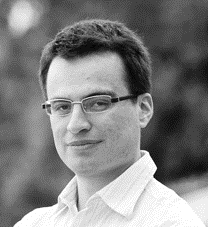
\includegraphics[scale=0.5]{Andres.png}
		%\caption{}
	}\hspace{0.5cm}%
	\subfloat[Rob Hyndman]{
		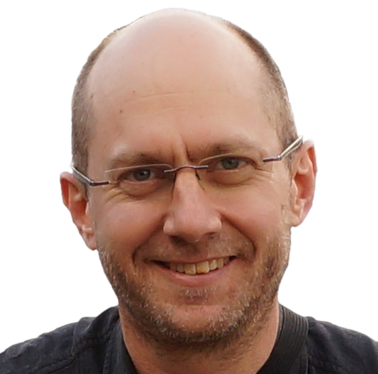
\includegraphics[scale=0.5]{Rob.png}
		%\caption{}
	}\hspace{0.5cm}%
	\subfloat[Kate Smith-Miles]{
		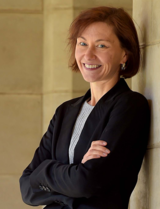
\includegraphics[scale=1.75]{Kate.png}
		\label{Kate}
		%\caption{}
	}%
  \end{figure}  
    \end{frame}

	\begin{frame}[label=figs1]
		\begin{figure}[b]
		\centering
		\tikzset{
			head/.style = {fill = none, label = center:\textsf{H}},
			tail/.style = {fill = none, label = center:\textsf{T}}}
		\scalebox{0.65}{\begin{tikzpicture}[
			scale = 1.5, transform shape, thick,
			every node/.style = {draw, circle, minimum size = 10mm},
			grow = down,  % alignment of characters
			level 1/.style = {sibling distance=3cm},
			level 2/.style = {sibling distance=4cm},
			level 3/.style = {sibling distance=2cm},
			level distance = 2.25cm]
			\node[shape = rectangle,
			minimum width = 6cm, minimum height = 1.5cm, font = \sffamily, rounded corners, fill={rgb:red,0;green,176;blue,80}] {About outlier detection};
	
			
			% Labels
		\end{tikzpicture}}
	\end{figure}
	
	\end{frame}

\begin{frame}{Outlier detection}
\begin{itemize}
    \item It means different things to different people
    \item What is the definition of an outlier?
    \item Hawkins :  an observation that deviates so much from other observations as to arouse suspicion that it was generated by a different mechanism
    \item We focus on ground truth when labelling outliers
\end{itemize}
\end{frame}

\begin{frame}{Ground truth as an outlier}
    \begin{itemize}
        \item Blue dot - an alien, red dots - humans
    \end{itemize}
    \begin{figure}
    \captionsetup[subfigure]{labelformat=empty}
     \centering
	\subfloat[Figure 1]{
		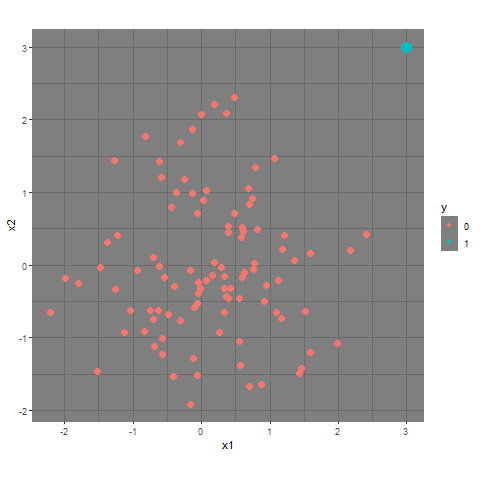
\includegraphics[width=0.48\textwidth]{example1.png}
		%\caption{}
	}%
	\subfloat[Figure 2]{
		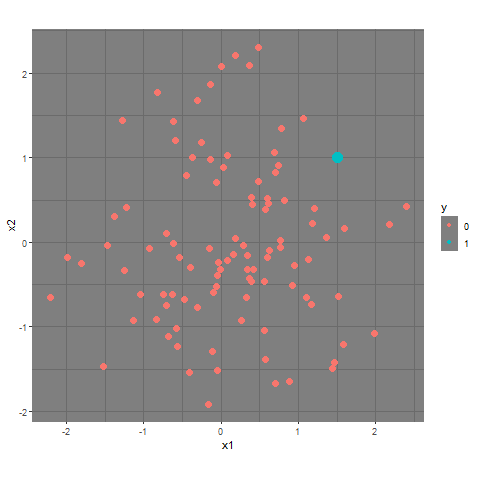
\includegraphics[width=0.48\textwidth]{example2.png}
		%\caption{}
	}
	\end{figure}
    
\end{frame}

\begin{frame}{Basic Mechanism}
\begin{itemize}
    \item data in $\mathbb{R}^n$ \vspace{0.5cm}
    \item A mapping $f : \mathbb{R}^n \to \mathbb{R} $  \vspace{0.5cm}
    \item such that outliers have different $f(x)$ compared with other points
\end{itemize}
\end{frame}

\begin{frame}{Disagreement between outlier methods}
       \begin{figure}
    \captionsetup[subfigure]{labelformat=empty}
     \centering
		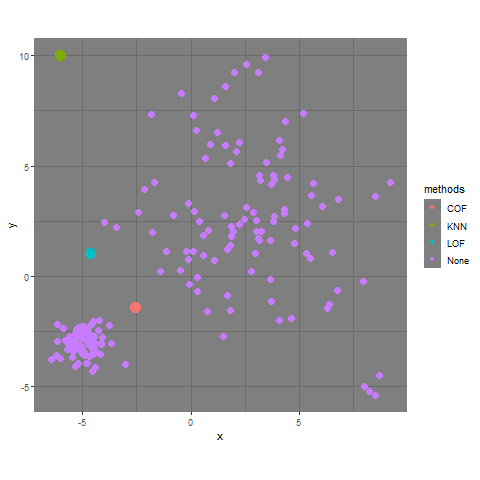
\includegraphics[width=0.8\textwidth]{example3.png}
	\end{figure}
\end{frame}



\begin{frame}{Research Question 1 - Algorithm Selection}
    \centering
    {\huge What is the best outlier detection } \\ \vspace{0.5cm}
    {\huge method for my problem?}
\end{frame}	

	\begin{frame}{More Questions - Normalization}
	\begin{itemize}
		\item Why normalize?
		\item Traditionally min-max normalization is used
		\item All columns are normalized to $[0, 1]$
		\item Other methods available - column by column
		\begin{itemize}
			\item Mean-SD
			\item Median-IQR
			\item Median-MAD
		\end{itemize}
		\vspace{1cm}		
		\item { \Large Why does it matter? }
		\end{itemize}
	\end{frame}

	\begin{frame}{Because . . .}
	\centering
	{\Huge Performance may suffer! }
	\end{frame}

	\begin{frame}{LOF - an Example}
	LOF - Local outlier factor \\
	(Breunig {\it et. al. })
	
	\begin{figure}[H]
	\centering
	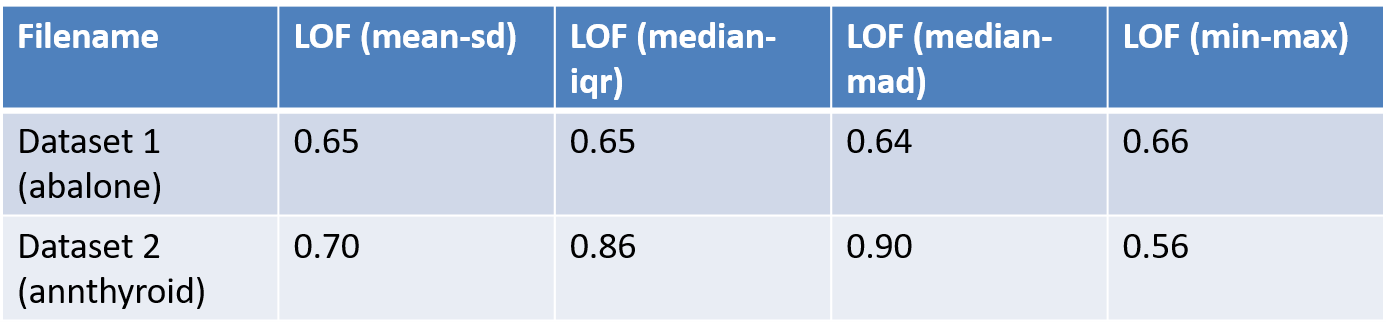
\includegraphics[scale=0.4]{LOF_Example.png}
	\end{figure}
	\end{frame}
	
	\begin{frame}{Research Question 2 - Normalization}
	 \centering
	  {\huge Can we understand the effect of}\\ \vspace{0.5cm}
	  {\huge normalization on outlier detection?}
	\end{frame}
	
		\begin{frame}[label=figsnorm]
		\begin{figure}[b]
		\centering
		\tikzset{
			head/.style = {fill = none, label = center:\textsf{H}},
			tail/.style = {fill = none, label = center:\textsf{T}}}
		\scalebox{0.65}{\begin{tikzpicture}[
			scale = 1.5, transform shape, thick,
			every node/.style = {draw, circle, minimum size = 10mm},
			grow = down,  % alignment of characters
			level 1/.style = {sibling distance=3cm},
			level 2/.style = {sibling distance=4cm},
			level 3/.style = {sibling distance=2cm},
			level distance = 2.25cm]
			\node[shape = rectangle,
			minimum width = 6cm, minimum height = 1.5cm, font = \sffamily, rounded corners, fill={rgb:red,0;green,176;blue,80}] {About Normalization};
			

			% Labels
		\end{tikzpicture}}
	\end{figure}
	
	\end{frame}

	
	\begin{frame}{WHY does normalization affect outlier detection?}
	\begin{itemize}
		\item Each axis is squashed/stretched differently
		\item Normalization changes distances
		\item Nearest neighbour structure changes
		\item Changes densities
		\vspace{1cm}
		\item {\Large Most outlier detection methods work on distances or densities}
		
	\end{itemize}
	\end{frame}

	\begin{frame}{Giving some notation \ldots }
	Let  $\mathbf{x}_i \in \mathbb{R}^d$. Normalizing it we get 
	\begin{equation*}\label{eq:norm1}
	\mathbf{x}^*_i = S^{-1}\left(\mathbf{x}_i - \mu \right) \, .
	\end{equation*}
	Here $\mathbf{x}^*_i$ is the normalized observation,  \\
	$\mu$ is minimum/mean/median  \\
	$S$ is a diagonal matrix containing column-wise range/standard deviation/IQR/MAD. \\
	 Let $S = \diag(s_1, s_2, s_3, \dots, s_d)$ and $\mathbf{w} = (1/s_1^2, 1/s_2^2, 1/s_3^2, \dots, 1/s_d^2)^T$. %If the range, standard deviation, IQR or MAD of a certain column $k$ is zero then we assign $1$ to $s_k$, i.e.\ we leave column $k$ unchanged. This assures  $S$ is  invertible. \margincomment{Shall we remove the zero denominator part? Need to say S is invertible.}  
	
	\begin{equation*}\label{eq:norm2}
	\dist(\mathbf{x}^*_i, \mathbf{x}^*_j) = \left\lVert S^{-1}\left(\mathbf{x}_i - \mathbf{x}_j \right) \right\rVert = \sqrt{ \left\langle \mathbf{w}\, , \left(\mathbf{x}_i - \mathbf{x}_j \right)^2 \right\rangle }
	\end{equation*}
	\end{frame}	

% 	\begin{frame}{Mathematically we show \ldots  }
%     \begin{itemize}
%         \item Depending on the normalization scheme
%         \begin{itemize}
%             \item Nearest neighbours change
%             \item Densities change
%         \end{itemize}
%         \item Normalization scheme can mask the true outliers and favour non-outliers  
%     \end{itemize}
%     \end{frame}
\end{darkframes}


    \begin{frame}{Proposition: Normalization scheme can mask the true outliers and favour non-outliers}
    \begin{figure}[!t]
	\centering
	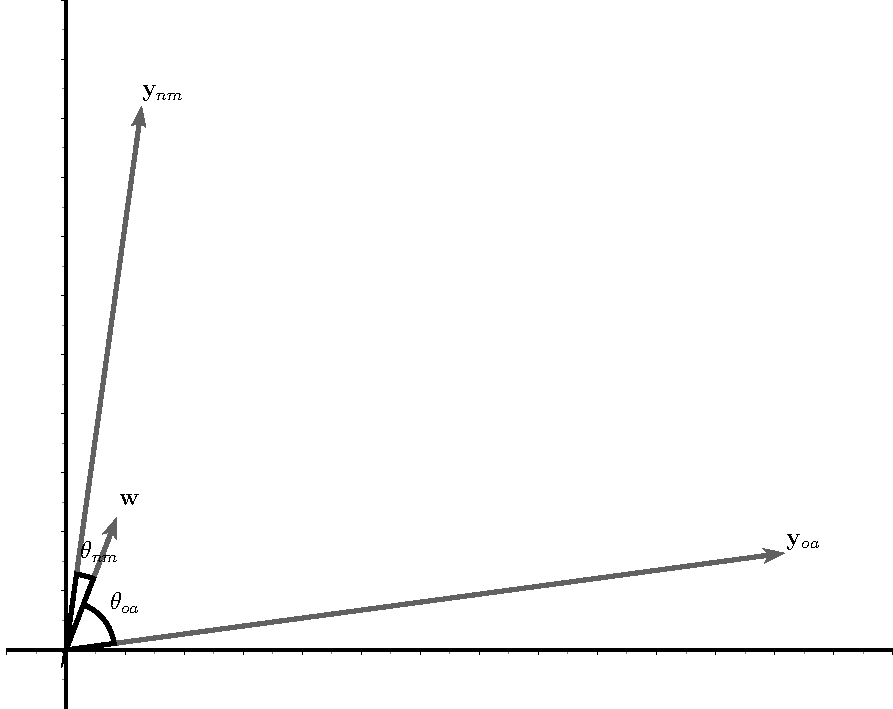
\includegraphics[clip=true, height=5cm]{Effect_of_w2.pdf}%width=0.40\textwidth, clip
	%\caption{The vectors $\bm{y}_{oa}$, $\bm{y}_{nm}$,  $\bm{w}$ with angles $\theta_{oa}$ and $\theta_{nm}$.}
	%\label{fig:effect_of_w}
\end{figure}
$$ \langle \bm{w}, \bm{y}_{oa} \rangle  < \langle \bm{w} , \bm{y}_{nm} \rangle \, , \text{with} \, \, $$ 
$$ \bm{y}_{oa}  = \left(\bm{x}_o - \bm{x}_a \right)^2 \,  \, \text{and} \, \,  \bm{y}_{nm}  = \left( \bm{x}_n - \bm{x}_m \right)^2\, . $$
 \end{frame}


\begin{darkframes}
    \begin{frame}{Any real data?}
        \centering
        {\huge We did a BIG experiment!}
    \end{frame}

  	\begin{frame}{Our experiment with real data}
 	\begin{itemize}
 		\item 12000+ datasets
 		\begin{itemize}
 			\item Around 200 sources, many variants
 		\end{itemize}
 		\item 4 normalization methods
 		\item 12 outlier detection methods
 		\item Meta-features
 		\begin{itemize}
 			\item Describe a dataset
 			\item Each dataset can be represented as a feature vector
 			\item A way to compare datasets
 			\item 346 meta-features
 		\end{itemize}
 		\item Matching outlier methods with datasets
 		\vspace{0.75cm}
 		\item A lot of time on the Monash Cluster 
 	\end{itemize}

 	\end{frame}	

 
 	
 	
    \begin{frame}{Normalization related results}
    \begin{equation*}
	y \sim \text{Out}  + \text{Norm} +  \text{Out} * \text{Norm} + (1|\text{Source}) \, .
\end{equation*}
    \begin{figure}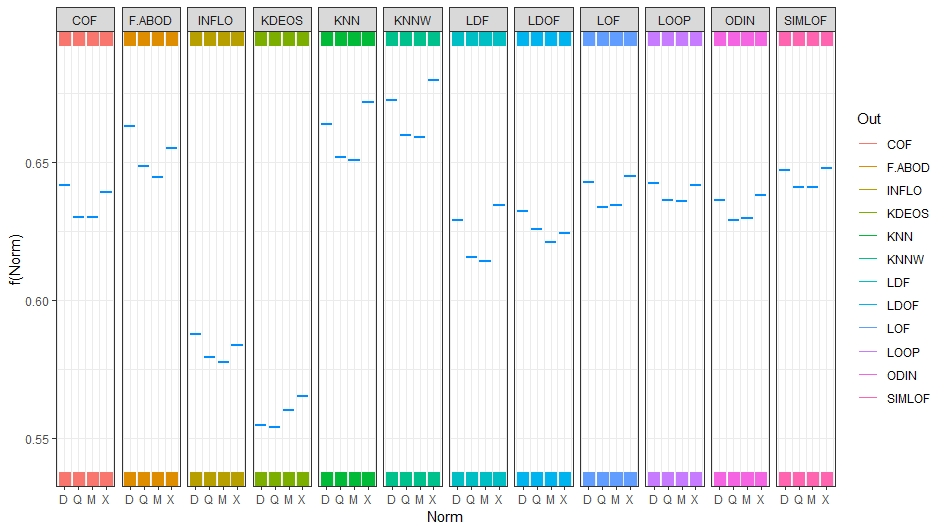
\includegraphics[scale=0.4]{fit3_Norm_Effect_By_Out.jpeg}
    \end{figure}
    \end{frame}	
    
    \begin{frame}{Observations from the plot}
    \begin{itemize}
        \item Generally Min-Max and Mean-SD perform better than Median-IQR and Median-MAD
        \item Min-Max and Mean-SD are similar, Median-IQR and Median-MAD are similar
        \item Best methods are KNNW, KNN and FAST ABOD
        \item KDEOS is the weakest method on average
    \end{itemize}
    \end{frame}
 		
     \begin{frame}{Why is Min-Max better?}
%   \begin{figure}
%     \captionsetup[subfigure]{labelformat=empty}
%      \centering
% 	\subfloat[Figure 1]{
% 		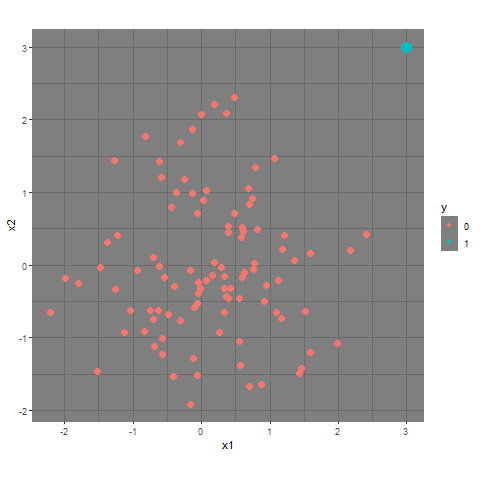
\includegraphics[width=0.48\textwidth]{example1.png}
% 		%\caption{}
% 	}%
% 	\subfloat[Figure 2]{
% 		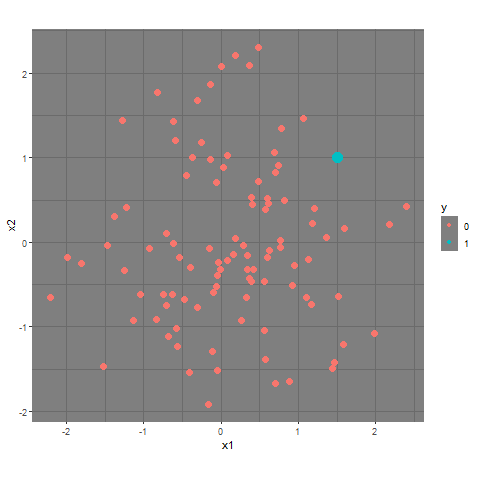
\includegraphics[width=0.48\textwidth]{example2.png}
% 		%\caption{}
% 	}
% 	\end{figure}     
    \begin{figure}
    \captionsetup[subfigure]{labelformat=empty}
     \centering
	\subfloat[Min-Max better]{
		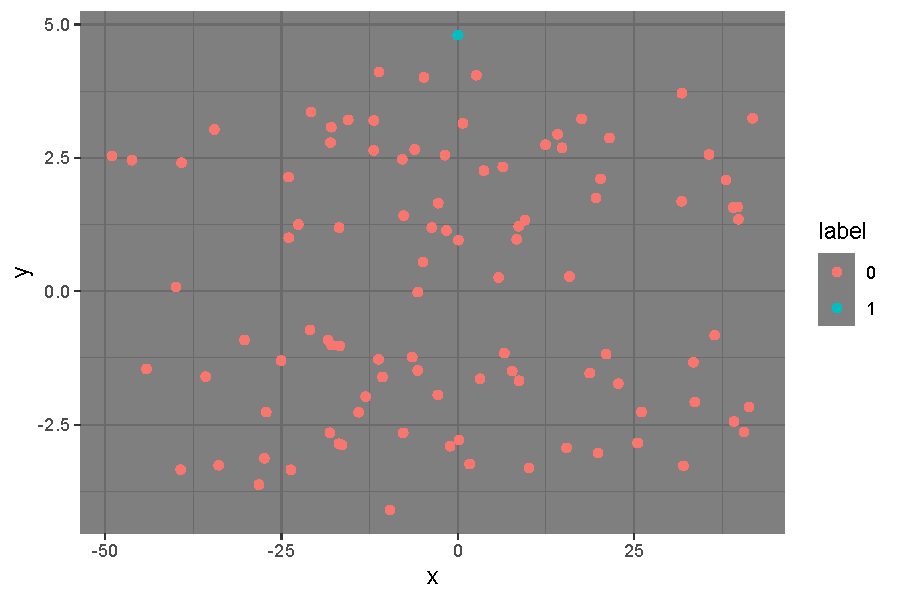
\includegraphics[width=0.48\textwidth]{Min_Max_Better.pdf}
		%\caption{}
	}%
	\subfloat[Median-IQR better]{
		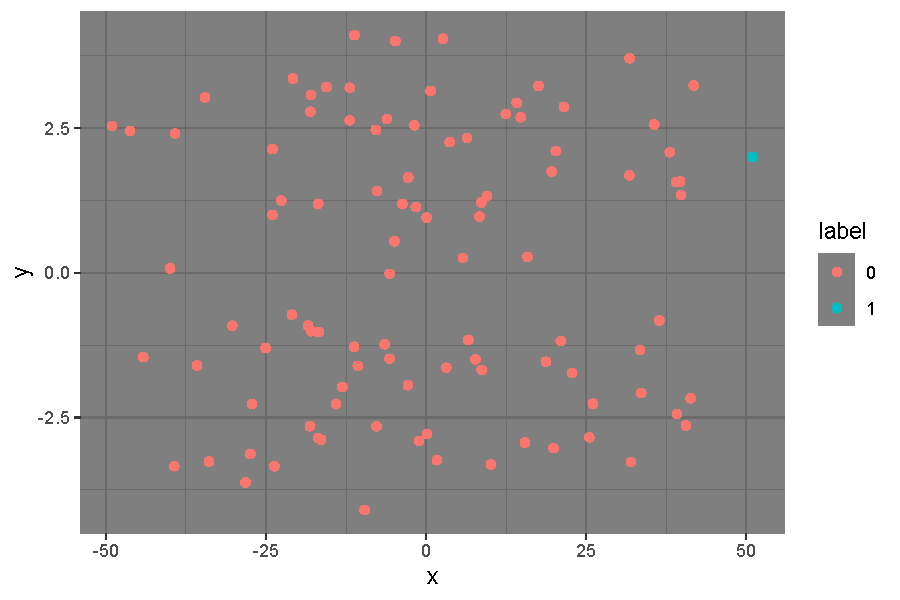
\includegraphics[width=0.48\textwidth]{Median_IQR_Better.pdf}
		%\caption{}
	}
	\end{figure}
	
    $\hspace{1cm} \mathbf{w} = \left( 1/100^2, 1/9^2\right )^T \hspace{1.5cm} \mathbf{w} = \left( 1/34^2, 1/5^2\right )^T $ 
    
    \begin{itemize}
        \item Min-Max favours outliers in directions other than the maximum range
        \item With higher dimensional datasets, it is more likely that outliers lie in  non-maximum range directions.
    \end{itemize}
	
% 	\begin{equation*}\label{eq:norm2}
% 	\dist(\mathbf{x}^*_i, \mathbf{x}^*_j) = \left\langle \mathbf{w}\, , \left(\mathbf{x}_i - \mathbf{x}_j \right) \right\rangle 
% 	\end{equation*}
    
    \end{frame}
 		
 	\begin{frame}{More results \ldots}
 	\begin{itemize}
 	    \item About 50\% of datasets prefer  Min-Max to Median-IQR - Median-IQR is a strong contender \\ \vspace{0.5cm}
 	    \item Some datasets are more sensitive to normalization than others  \\ \vspace{0.5cm}
 	    \item Some outlier methods are more sensitive to normalization than others
 	    
 	\end{itemize}
 	    
 	\end{frame}	
 	\begin{frame}{Takeaway}
 	    \begin{itemize}
 			\item 	Normalization is an important ``parameter'' of outlier detection techniques.
 			\vspace{0.5cm}
 			\item  Fixing the normalization method has its consequences.
 			\vspace{0.5cm}
 			\item  Find the best normalization that suits the dataset.
 		\end{itemize}
 		 
 	\end{frame}
 		
 	\begin{frame}[label=figsnorm]
		\begin{figure}[b]
		\centering
		\tikzset{
			head/.style = {fill = none, label = center:\textsf{H}},
			tail/.style = {fill = none, label = center:\textsf{T}}}
		\scalebox{0.65}{\begin{tikzpicture}[
			scale = 1.5, transform shape, thick,
			every node/.style = {draw, circle, minimum size = 10mm},
			grow = down,  % alignment of characters
			level 1/.style = {sibling distance=3cm},
			level 2/.style = {sibling distance=4cm},
			level 3/.style = {sibling distance=2cm},
			level distance = 2.25cm]
			\node[shape = rectangle,
			minimum width = 6cm, minimum height = 1.5cm, font = \sffamily, rounded corners, fill={rgb:red,0;green,176;blue,80}] {Algorithm Selection};
			

			% Labels
		\end{tikzpicture}}
	\end{figure}
	
	\end{frame}
 		
 \begin{frame}{Research Question 1}
 	\begin{figure}[!t]
 	\centering
 	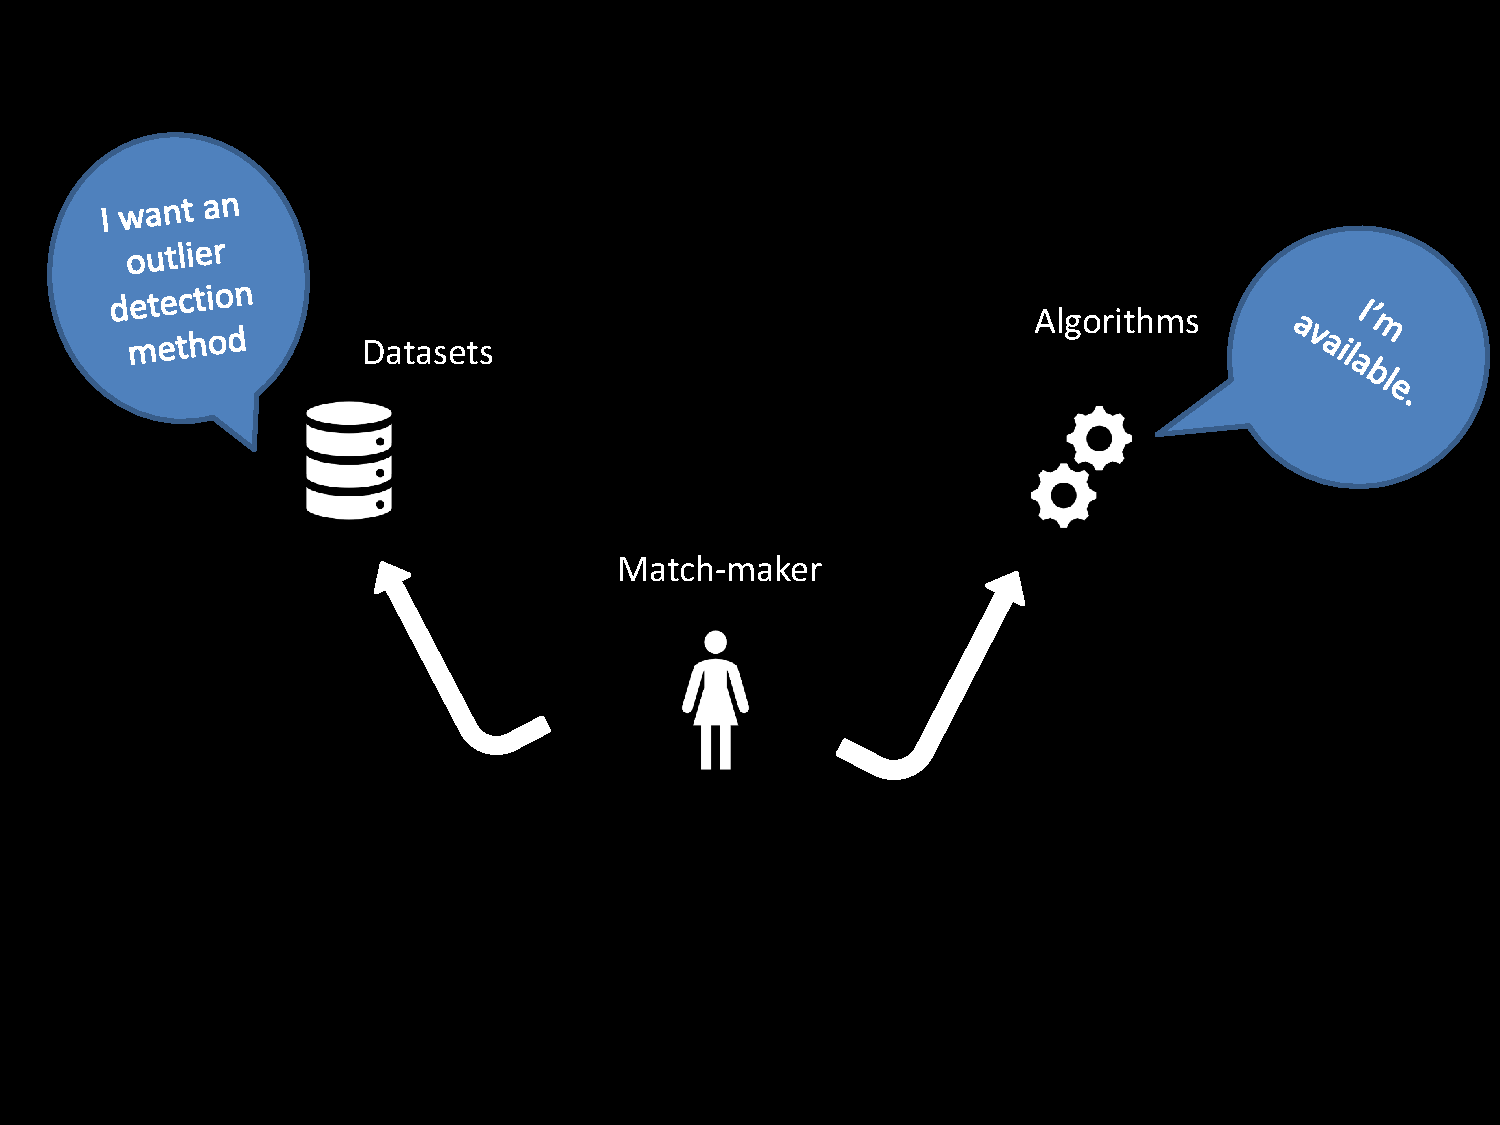
\includegraphics[clip=true, height=6.45cm]{match_maker.pdf}%width=0.40\textwidth, clip
   	\end{figure}
 	\end{frame}	
 	
 	\begin{frame}[label=process1]
 	 \centering
        \begin{tikzpicture}[node distance=2cm]
			\node(data)[process] {Datasets};
			\node(algo)[io,below of=data, xshift=-2cm]{Algorithms};
			\node(output)[process, below of=algo]{Output};
			\node(goodperf)[process, below of=output, minimum width=3cm, text width=3cm, xshift=2cm]{Good or bad performance};
			\node(meta)[process, below of=data, xshift=2cm]{Meta-features};
			\draw [arrow] (data) -- (algo);
			\draw [arrow] (algo) -- (output);
			\draw [arrow] (data) -- (meta);
			\draw [arrow] (output) -- (goodperf);
			%\draw [arrow, color=red] (meta) --  (goodperf);
			% Labels
		\end{tikzpicture}
    
	\end{frame}
 	
 		\begin{frame}[label=process2]
 	 \centering
        \begin{tikzpicture}[node distance=2cm]
			\node(data)[process] {Datasets};
			\node(algo)[io,below of=data, xshift=-2cm]{Algorithms};
			\node(output)[process, below of=algo]{Output};
			\node(goodperf)[process, below of=output, minimum width=3cm, text width=3cm, xshift=2cm]{Good or bad performance};
			\node(meta)[process, below of=data, xshift=2cm]{Meta-features};
			\node(rforest)[io,below of=meta, minimum width=2cm, text width=2cm]{Randomforest classifier};

			\draw [arrow] (data) -- (algo);
			\draw [arrow] (algo) -- (output);
			\draw [arrow] (data) -- (meta);
			\draw [arrow] (output) -- (goodperf);
			\draw [arrow, color=red] (meta) --  (rforest);
			\draw [arrow, color=red] (rforest) --  (goodperf);
			% Labels
		\end{tikzpicture}
    
	\end{frame}
 		
 	
   \begin{frame}{Meta-features}
        \begin{itemize}
            \item Simple features 
            \begin{itemize}
                \item Number of obs., attributes, binary attributes, \ldots
            \end{itemize}
            \item Statistical features
            \begin{itemize}
                \item skewness, kurtosis, mean to sd \ldots
            \end{itemize}
            \item Information theoretic features
              \begin{itemize}
                \item entropy, mutual information,  \ldots
            \end{itemize}
            \item Density based features
              \begin{itemize}
                \item DBSCAN, Kernel density estimates \ldots
            \end{itemize}
            \item Residual based features
            \item Graph based features
        \end{itemize}
    \end{frame}
 \begin{frame}{Breakdown of features}
 \begin{table}[!t]
	\centering

	\footnotesize
	\begin{tabular}{p{3.5cm}p{3cm}}
		\toprule
		Feature category       & Number of features \\
		\midrule
		 Generic : Simple, Statistical and Information theoretical & $25$               \\ % It would be nice to have the actual breakdown of these classes
		Density based          & $77$               \\
		Residual based         & $35$               \\
		Graph based            & $41$               \\
		\midrule
		Total                  & 178                   \\
		\bottomrule
	\end{tabular}
	\label{tab:featureCount}
\end{table}
 We use outlier labels to compute some features.
 \end{frame}	
 	
\begin{frame}{Predict performance using 10 fold CV}
    \begin{table}[!t]
	\centering
	\footnotesize
	\begin{tabular}{p{3.5cm}p{3cm}p{3cm}}
		\toprule
		Outlier detection method & Default accuracy(\%)  & Prediction accuracy(\%)       \\
		\midrule
		COF                      & 75.58      & 83.48                   \\
		FAST ABOD                & 67.77      & 86.07                    \\
		INFLO                    & 83.22      & 89.29                    \\
		KDEOS                    & 90.96      & 92.81                    \\
		KNN                      & 68.16      & 86.56                    \\
		KNNW                     & 67.13      & 86.13                     \\
		LDF                      & 75.65      & 85.28                    \\
		LDOF                     & 80.08      & 87.36                   \\
		LOF                      & 74.63      & 84.07                    \\
		LOOP                     & 77.19      & 85.88                     \\
		ODIN                     & 79.09      & 87.00                    \\
		SIMLOF                   & 75.85      & 85.21                    \\
		\bottomrule
	\end{tabular}
	\label{table:predOutPerf}
\end{table}
\end{frame}

\begin{frame}[label=process3]
 	 \centering
        \begin{tikzpicture}[node distance=2cm]
			\node(data)[process] {Datasets};
			\node(algo)[io,below of=data, xshift=-2cm]{Algorithms};
			\node(output)[process, below of=algo]{Output};
			\node(goodperf)[process, below of=output, minimum width=3cm, text width=3cm, xshift=2cm]{Good or bad performance};
			\node(meta)[process, below of=data, xshift=2cm]{Meta-features};
			\node(featselect)[io,right of=meta, xshift=2cm,minimum width=2cm, text width=2cm]{Feature selection};
			\node(projection)[io,below of=featselect, minimum width=2cm, text width=2cm]{Project to 2D};
			\node(instsp)[process, below of=projection]{Instance space};
			
;			\draw [arrow] (data) -- (algo);
			\draw [arrow] (algo) -- (output);
			\draw [arrow] (data) -- (meta);
			\draw [arrow] (output) -- (goodperf);
		    \draw [arrow] (meta) -- (featselect);
		    \draw [arrow] (featselect) -- (projection);
		    \draw [arrow](projection) --(instsp);
		    \draw [arrow](output) --(projection);
			
			% Labels
		\end{tikzpicture}
    
\end{frame}  

\begin{frame}{Feature selection}
\begin{itemize}
    \item Discard features that has less than 30\% unique values ( 135 features)
    \item Select the highest correlated features with performance ( 26 features)
    \item Group features, by $k$-means clustering using $1 - |\rho|$. (7 clusters)
    \item Total feature combinations : 2352
    \item For each feature combination, fit a random forest on a 2D PC space for each algorithm 
    \item The best combination is the one with the lowest average out of bag error
\end{itemize}
\end{frame} 

\begin{frame}{Chosen features}
\begin{itemize}
    \item Mean\_Entropy\_Attr (generic) 
    \begin{itemize}
        \item     Mean entropy of attributes
    \end{itemize}
    \item IQR\_TO\_SD\_95 (generic)   
      \begin{itemize}
        \item     95\% of IQR to Standard deviation of attributes
    \end{itemize}
	\item OPO\_Res\_ResOut\_Median (residual) 
	\begin{itemize}
	    \item 	Median proxi-outlier residuals/ median non-PO residuals
	\end{itemize}
	\item OPO\_Res\_Out\_Mean (residual) 
	\begin{itemize}
	    \item 	Mean of outlier residuals / mean of non-outlier residuals
	\end{itemize}
	\item OPO\_Den\_Out\_95P (density) 
	\begin{itemize}
	    \item 	95\% of density of non-outliers / 95\% of density of outliers
	\end{itemize}
	\item OPO\_GDeg\_PO\_Mean (graph) 
	\begin{itemize}
	    \item 	Mean graph degree inner points/mean graph degree non-inner points
	\end{itemize}
	\item OPO\_GDeg\_Out\_Mean (graph) 
	\begin{itemize}
	    \item 	Mean graph degree of outliers / mean graph degree of non-outliers
	\end{itemize}
\end{itemize}
    
\end{frame}
    
\begin{frame}{The projection}
\begin{itemize}
    \item PBLDR : Prediction Based Linear Dimensionality Reduction 
    \item Finds a projection with most linear trends in algorithm performance and feature values
\end{itemize}
\begin{equation*}
	\textbf{Z} =
	\left[
		\begin{array}{rr}
		-0.0862 &   -0.2078 \\ %3
		 0.1737 &    0.1845 \\ %6
		-0.0460 &   -0.2847 \\ %1
		-0.0938 &   -0.2025 \\ %4
		 0.1202 &    0.0378 \\ %2
		 0.1854 &   -0.0822 \\ %5
		 0.3543 &   -0.1325 \\ %7
		\end{array}%
		\right]^{\top} 
	\left[
		\begin{array}{l} 
			\text{\small{Mean\_Entropy\_Attr}}      \\ %3
			\text{\small{IQR\_TO\_SD\_95}}          \\ %6
			\text{\small{OPO\_Res\_ResOut\_Median}} \\ %1
			\text{\small{OPO\_Res\_Out\_Mean}}      \\ %4
			\text{\small{OPO\_Den\_Out\_95P}}       \\ %2
			\text{\small{OPO\_GDeg\_PO\_Mean}}      \\ %5
			\text{\small{OPO\_GDeg\_Out\_Mean}}     \\ %7
		\end{array}
		\right]
			\label{eq:projection_model}
\end{equation*}
\end{frame}    

\begin{frame}{Instance space}
    \begin{figure}
        \centering
        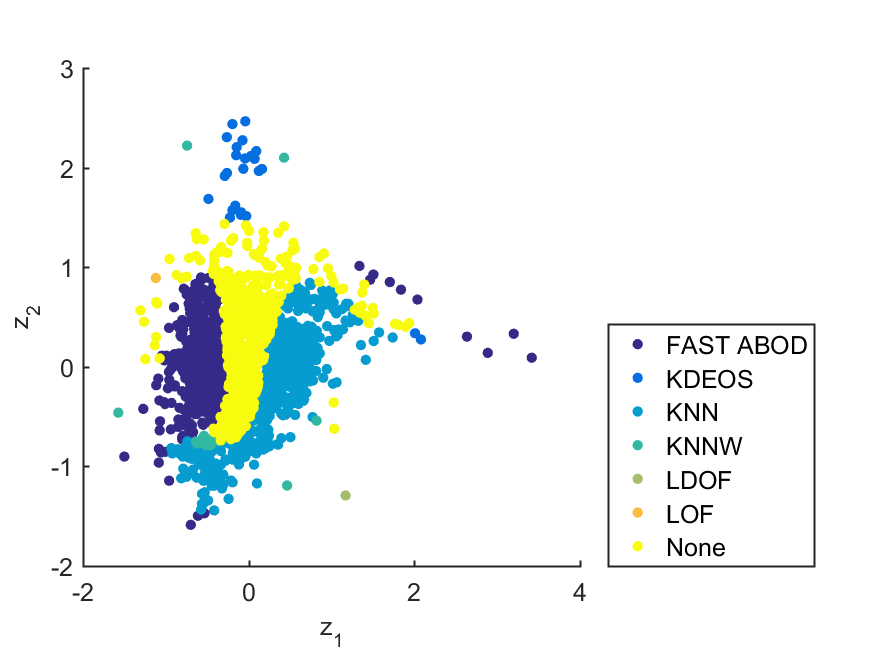
\includegraphics[scale= 0.6]{svm_pbldr_family.png}
    \end{figure}
\end{frame}


\begin{frame}{Takeaway}
\begin{itemize}
    \item No outlier method is superior to all other methods \\ \vspace{0.5cm}
    \item Need to find the suitable method for a given problem \\ \vspace{0.5cm}
    \item We find the strengths and weaknesses via instance space methodology
\end{itemize}
    
\end{frame}

    \begin{frame}
    \begin{figure}[b]
		\centering
		\tikzset{
			head/.style = {fill = none, label = center:\textsf{H}},
			tail/.style = {fill = none, label = center:\textsf{T}}}
		\scalebox{0.65}{
		\begin{tikzpicture}[
			scale = 1.5, transform shape, thick,
			every node/.style = {draw, circle, minimum size = 10mm},
			grow = down,  % alignment of characters
			level 1/.style = {sibling distance=3cm},
			level 2/.style = {sibling distance=4cm},
			level 3/.style = {sibling distance=2cm},
			level distance = 2.25cm
			]
			\node[shape = rectangle,
			minimum width = 4cm, font = \sffamily, rounded corners, fill={rgb:red,0;green,176;blue,80}] {Outlier Detection}% fill=black!60!green
			child { node[shape = rectangle, draw, line width = 1pt,
				minimum width = 4cm, xshift=-1.5cm, rounded corners, fill={rgb:red,0;green,176;blue,80}] (Start){Normalization}
			}
			child { node[shape = rectangle, draw, line width = 1pt,
				minimum width = 4cm, xshift=1.5cm, rounded corners, fill={rgb:red,0;green,176;blue,80}] (Start){Algorithm Selection}
			};
			
			% Filling the root (Start)
			\begin{scope}[on background layer, rotate=30]
			\fill[head] (Start.base) ([xshift = 0mm]Start.east) arc (0:180:5mm)
			-- cycle;
			\fill[tail] (Start.base) ([xshift = 0pt]Start.west) arc (180:360:5mm)
			-- cycle;
			\end{scope}
			
			% Labels
		\end{tikzpicture}}
	\end{figure}
 	\end{frame}
 	
 	\begin{frame}{Thank you!}
 	\centering
 	\begin{itemize}
 		\item R package \textit{outselect} at https://github.com/sevvandi/outselect
 		\item Datasets at https://monash.figshare.com/articles/Datasets12338zip/7705127/4
 		\item  Pre-print on research gate: On normalization and algorithm selection for unsupervised outlier detection 
 	\end{itemize}
 
 		
 	\end{frame}
  	\end{darkframes}
\end{document}
